\documentclass[aps,prm,reprint,onecolumn,superscriptaddress]{revtex4-2}
\usepackage{amsmath,amssymb}
\usepackage{graphicx}
\usepackage{hyperref}
\usepackage{booktabs}

\begin{document}

\title{What harmonic phonon calculations capture --- and miss --- about thermal conductivity}

\author{Alexandru Toader}
\affiliation{Independent researcher, Buz\u{a}u, Romania}
\email{toader\_alexandru@yahoo.com}

\begin{abstract}
Harmonic force constants predict lattice thermal conductivity with cross-validated $R^2 = 0.86$--$0.89$ across 751 crystalline solids spanning 4.7 orders of magnitude in $\kappa$, using 14 standard phonon descriptors. The plateau persists across linear, ensemble, and neural network models and does not improve with additional engineered features. The remaining variance is primarily correlated with cubic coupling strength $|V_3|^2$, which is weakly coupled to harmonic bond stiffness after controlling for atomic mass (partial $r = -0.05$). The prediction ceiling arises not because models are insufficient, but because anharmonic scattering is approximately decoupled from harmonic structure. Rigid oxides and layered compounds illustrate this decoupling most clearly.
\end{abstract}

\maketitle

\section{Introduction}

Lattice thermal conductivity $\kappa$ is a central quantity in thermal management of electronics~\cite{cahill2003}, thermoelectric energy conversion~\cite{snyder2008}, and thermal barrier coating design~\cite{clarke2005}. First-principles prediction of $\kappa$ through the phonon Boltzmann transport equation (BTE) with anharmonic (third-order) force constants is now well established~\cite{li2014,togo2015} and agrees with experiment to within 10--20\% for many crystalline solids~\cite{lindsay2020}. However, the computational cost of obtaining third-order force constants remains substantial --- typically requiring hundreds of supercell calculations per material --- which limits the throughput of BTE-based screening~\cite{togo2023}.

Harmonic (second-order) force constants are considerably cheaper to obtain, requiring only a single set of displaced-atom calculations. From the harmonic dynamical matrix one can extract phonon dispersion relations, sound velocities, Debye temperatures, phonon density of states, and derived quantities such as the three-phonon phase space volume~\cite{lindsay2008}. Several studies have used these harmonic properties to estimate $\kappa$, either through analytical models~\cite{slack1973,morelli2006} or machine-learning approaches~\cite{carrete2014,juneja2019}, with reported accuracy varying from $R^2 \approx 0.6$ to $R^2 \approx 0.9$ depending on the feature set, model complexity, and dataset. These studies have focused on improving predictive accuracy. What has received less attention is the characterization of the residual: what physical information is absent from harmonic models, and whether any inexpensive descriptor can recover it. If the remaining ${\sim}10\%$ of variance reflects missing physics --- specifically information contained in higher-order force constants --- then improving harmonic models is fundamentally limited.

We address this question on 751 materials from PhononDB~\cite{togo2023} for which both harmonic force constants and BTE-computed $\kappa$ at 300~K are available. We train models of increasing complexity, characterize the plateau, and correlate the harmonic residual with anharmonic quantities available for a 231-material subset. We find that the residual is primarily correlated with cubic anharmonic strength, which is weakly coupled to harmonic bond stiffness, supporting an approximate factorization of $\kappa$ into contributions that depend on different derivatives of the interatomic potential.

\section{Data and methods}

\subsection{Dataset}

We use 751 materials from PhononDB~\cite{togo2023} that have both harmonic force constants (FORCE\_SETS from phonopy~\cite{togo2015scr}) and lattice thermal conductivity computed via the linearized BTE at 300~K (phono3py~\cite{togo2015}). Three materials with known BTE convergence artifacts are excluded, as are materials with unresolved sound velocities. Ten additional materials are excluded because the electronegativity contrast feature requires at least two distinct elements with known Pauling electronegativities (B, two Si polymorphs, three Hg compounds, four Yb compounds). The dataset spans six crystal systems: orthorhombic ($N = 209$), monoclinic (175), cubic (136), trigonal (104), tetragonal (85), and hexagonal (42).

\subsection{Harmonic features}

From the harmonic force constants of each material we extract 14 features:

\begin{itemize}
\item \textbf{Sound velocities} (3): longitudinal $v_\mathrm{LA}$, transverse $v_\mathrm{TA}$, and the Brillouin-zone-averaged squared velocity $\mathrm{sv2} = \sum_\mathbf{q} v^2(\mathbf{q}) / N_\mathbf{q}$.
\item \textbf{Debye temperature} (1): $\theta_D$ computed from the second moment of the phonon density of states.
\item \textbf{Phase space volume} (1): $W$, the weighted three-phonon scattering phase space~\cite{lindsay2008}, computable from the harmonic dispersion alone.
\item \textbf{Spectral shape} (5): spectral spread, maximum frequency gap, fraction of sv2 below median frequency, spectral entropy, and DOS bandwidth ratio.
\item \textbf{Structural} (4): average atomic mass, electronegativity contrast, mean diagonal force constant ($f_\mathrm{c,mean}$), and interaction range.
\end{itemize}

All 14 features are computable from FC2 in seconds per material. The target variable is $\log_{10}(\kappa_\mathrm{BTE})$. As a robustness check, we verify that adding 19 engineered features yields minimal improvement in nonlinear models (Sec.~\ref{sec:accuracy}).

\subsection{Models}

We train three model families: (1) Ridge regression (linear baseline), (2) gradient boosting (500 trees, max depth 4), and (3) a neural network (MLPRegressor, layers 256-128-64). All are evaluated by 10-fold cross-validation with a fixed random seed. Feature ablation adds feature groups incrementally: sound velocities $\to$ Debye temperature $\to$ spectral shape $\to$ structural descriptors $\to$ phase space volume.

\subsection{Anharmonic data}

RTA calculations are available for 240 materials in PhononDB; of these, 231 overlap with the main dataset after exclusion criteria. From the RTA results we extract the BZ-averaged phonon scattering rate $\Gamma$, weighted by each mode's contribution to thermal conductivity ($C_\mathbf{q} v_\mathbf{q}^2 / \sum C_\mathbf{q} v_\mathbf{q}^2$) as computed by phono3py~\cite{togo2015}. We define the effective cubic coupling strength as $|V_3|^2 \equiv \Gamma/W$, which isolates the coupling contribution from the kinematic phase space. This is a transport-weighted proxy rather than a direct FC3 norm, but captures the component of scattering relevant for thermal transport. These quantities are used for residual analysis only. The ratio $\kappa_\mathrm{BTE}/\kappa_\mathrm{RTA}$ serves as a direct test of whether harmonic features carry any anharmonic information.

\section{Results}

\subsection{Harmonic prediction accuracy}
\label{sec:accuracy}

With 14 features, Ridge regression achieves $R^2 = 0.86 \pm 0.04$, gradient boosting $R^2 = 0.88 \pm 0.02$, and the neural network $R^2 = 0.89 \pm 0.03$ on 751 materials spanning $\kappa$ from 0.01 to 449~W/mK (Fig.~\ref{fig:ceiling}). Feature ablation on Ridge reveals a clear hierarchy: sound velocities alone yield $R^2 = 0.61$; adding Debye temperature gives 0.63; spectral shape brings 0.79; structural descriptors reach 0.83; and including phase space volume $W$ completes the set at 0.86. The marginal contribution of $W$ ($+0.02$) is context-dependent, consistent with its role as a kinematic complement to sound velocity.

Extending to 33 descriptors (+19 engineered features), Ridge improves to $R^2 = 0.89$ and the neural network to $R^2 = 0.90$, a gain of less than 0.02 over the 14-feature baseline. A learning curve analysis confirms that the plateau is not data-limited: all three models largely saturate by $N \approx 400$, with gains of less than 0.01 between $N = 400$ and $N = 751$ (Fig.~\ref{fig:learning}).

\subsection{Characterizing the residual}

To determine whether the harmonic residual contains anharmonic information, we test two quantities on the 231-material RTA overlap.

First, we ask whether harmonic features predict the ratio $\log(\kappa_\mathrm{BTE}/\kappa_\mathrm{RTA})$, which isolates the beyond-RTA anharmonic correction. All three models give negative $R^2$ (Ridge $-0.39$, GB $-2.12$, MLP $-1.48$), substantially worse than predicting the mean. The anharmonic correction carries no detectable harmonic signal within the tested model classes.

Second, we correlate the cross-validated harmonic residual with the anharmonic scattering rate $\Gamma$. Using a 5-feature baseline (sv2, mass, $f_\mathrm{c,mean}$, $\theta_D$, $W$), the residual correlates with $\log(\Gamma)$ at $r = -0.54$. The full 14-feature model yields $r = -0.29$ ($p < 10^{-4}$) --- the reduction reflects removal of harmonic variance, not loss of anharmonic signal. Since $W$'s partial correlation with the residual is negligible ($r = -0.01$ after mass control), the residual's correlation with $\Gamma$ is consistent with a dominant contribution from cubic coupling strength $|V_3|^2$ (Fig.~\ref{fig:residual}).

The residual shows no significant dependence on material class (ANOVA $p = 0.07$ across ten dominant-element groups) and no significant autocorrelation (Durbin-Watson 1.78--2.16).

\subsection{Weak coupling between stiffness and asymmetry}

The correlation between $\log(f_\mathrm{c,mean})$ and $\log(|V_3|^2)$ is $r = +0.09$ ($p = 0.15$, $n = 231$). Controlling for atomic mass gives partial $r = -0.05$ ($p = 0.46$). A Spearman rank correlation confirms the same pattern: $\rho = +0.17$ before mass control, $\rho = +0.04$ after. At this sample size, correlations $|r| > 0.13$ would be detectable at the 95\% level (Fig.~\ref{fig:stiffness}).

Conditioning on additional harmonic features (sv2, $\theta_D$) reveals a moderate conditional correlation (partial $r = -0.28$, $p < 10^{-4}$). This is physically expected --- at fixed phonon structure, stiffer bonds tend to be more symmetric --- but reflects redundancy within the harmonic descriptor space rather than access to anharmonic information: removing $f_\mathrm{c,mean}$ from the 14-feature model changes the residual's correlation with $|V_3|^2$ by less than 0.005. This statistical independence is the structural origin of the observed prediction ceiling: bond stiffness does not predict anharmonic scattering strength.

\subsection{Material classes at the boundary}

Two material classes exhibit systematic deviations that illustrate the stiffness-asymmetry decoupling (Fig.~\ref{fig:outliers}). These examples are illustrative rather than statistically representative.

\textbf{Rigid oxides} (TiO$_2$, ReO$_3$, ZrO$_2$, SnO$_2$; $n = 4$): high bond stiffness but high $|V_3|^2$ (1.36 standard deviations above mean, Mann-Whitney $p = 0.006$). The small sample size limits statistical power, but the direction is consistent: rigid metal-oxygen frameworks with soft tilting modes generate strong anharmonic scattering. The harmonic model overpredicts $\kappa$ for all four.

\textbf{Layered compounds} (GaSe (two polymorphs), GaS, GaTe, WS$_2$, MoS$_2$, WSe$_2$, BiI; $n = 8$): low average stiffness but low $|V_3|^2$ (1.60 standard deviations below mean, $p < 0.001$). The in-plane bonding is covalent and symmetric, suppressing anharmonic scattering despite low average stiffness. The harmonic model underpredicts $\kappa$.

Both deviations survive mass control (rigid oxide $p = 0.005$, layered $p < 0.001$).

\subsection{Oracle bound on the harmonic ceiling}

Harmonic features jointly predict $|V_3|^2$ at cross-validated $R^2 = 0.70$, but adding this prediction to the $\kappa$ model yields zero lift ($\Delta R^2 < 0.001$) --- the FC2~$\to$~$|V_3|^2$ channel is already fully exploited. The ceiling is set by the residual variance of $|V_3|^2$ that FC2 cannot access. Adding the true $|V_3|^2$ residual (an oracle test) improves $R^2$ by $+0.04$ (from 0.79 to 0.83 on the 231-material subset), and no tested structural descriptor correlates with this residual (all $|r| < 0.04$). Breaking the harmonic ceiling requires explicit third-order force constant information.

\section{Discussion}

\subsection{Interpretation}

The kinetic expression $\kappa = \frac{1}{3} \sum_\mathbf{q} C(\mathbf{q})\, v^2(\mathbf{q})\, \tau(\mathbf{q})$ separates naturally into harmonic quantities ($C$, $v$) and anharmonic coupling ($\tau$). In the BZ-averaged form, this separation can be made explicit in a minimal form:
\begin{equation}
\kappa \approx A \cdot \mathrm{sv2} \cdot \Gamma^{-1}
\end{equation}
A two-variable regression gives in-sample $R^2 = 0.78$ (cross-validated $R^2 = 0.73 \pm 0.17$) with coefficients $a = +1.11$, $b = -0.80$, consistent with the physical expectation ($a \approx +1$, $b \approx -1$).

\subsection{Tested descriptors that do not bridge the gap}

We evaluated several candidate descriptors: Morse-potential Gr\"uneisen parameter ($\rho = +0.22$ with residual, $R^2$ lift $= +0.008$), inverse group velocity and spectral skewness proxies (not significant), and element-based $|V_3|^2$ proxies (cross-validated $R^2 = 0.55$ for $|V_3|^2$ prediction, $\kappa$ lift $= +0.004$). None meaningfully reduced the harmonic residual.

While prior work has focused on improving $\kappa$ prediction from harmonic descriptors~\cite{carrete2014,juneja2019}, the present results suggest that such improvements are fundamentally bounded unless anharmonic information is introduced explicitly.

\subsection{Practical implications}

For high-throughput screening where ranking matters more than absolute accuracy, harmonic models provide useful $\kappa$ predictions with median relative error ${\sim}33\%$. For higher precision, anharmonic calculations remain necessary. The $R^2 \approx 0.89$ level offers a practical benchmark: further effort is better directed toward computing FC3 for selected candidates than toward engineering richer harmonic descriptors.

\subsection{Structural perspective}

The weak coupling between harmonic mode structure and anharmonic scattering rates has a structural interpretation. On lattice models with uniform stiffness, acoustic eigenvectors are invariant to overall stiffness scaling --- only eigenfrequencies change. Scattering rates involve third-order coupling projected onto these eigenvectors and constitute independent information. The approximate separability observed here is consistent with this picture. More generally, second- and third-order force constant properties describe different aspects of the potential energy surface (curvature vs.\ asymmetry) that are not constrained to co-vary.

\section{Conclusion}

Fourteen standard harmonic descriptors predict lattice thermal conductivity with $R^2 = 0.86$--$0.89$ on 751 crystalline solids spanning 4.7 orders of magnitude in $\kappa$. The remaining variance is primarily correlated with cubic anharmonic strength, which is weakly coupled to harmonic bond stiffness after controlling for atomic mass. An oracle test confirms that the unpredictable component of $|V_3|^2$ is the binding constraint, and no tested inexpensive descriptor accesses it. These findings suggest that the accuracy of harmonic $\kappa$ models is largely governed by the approximate separability of propagation and scattering physics, and help delineate when anharmonic calculations become necessary.

\section*{Data availability}

All harmonic features, BTE thermal conductivities, and analysis scripts are available at [repository URL]. The underlying force constants are from PhononDB~\cite{togo2023}.

\begin{thebibliography}{13}
\bibitem{cahill2003} D.~G. Cahill \textit{et al.}, J. Appl. Phys. \textbf{93}, 793 (2003).
\bibitem{snyder2008} G.~J. Snyder and E.~S. Toberer, Nat. Mater. \textbf{7}, 105 (2008).
\bibitem{clarke2005} D.~R. Clarke and S.~R. Phillpot, Mater. Today \textbf{8}, 22 (2005).
\bibitem{li2014} W.~Li \textit{et al.}, Comput. Phys. Commun. \textbf{185}, 1747 (2014).
\bibitem{togo2015} A.~Togo, L.~Chaput, and I.~Tanaka, Phys. Rev. B \textbf{91}, 094306 (2015).
\bibitem{lindsay2020} L.~Lindsay, in \textit{Nanoscale Energy Transport} (IOP, 2020).
\bibitem{togo2023} A.~Togo, L.~Chaput, T.~Tanaka, and I.~Tanaka, J. Phys.: Condens. Matter \textbf{35}, 353001 (2023).
\bibitem{lindsay2008} L.~Lindsay and D.~A. Broido, J. Phys.: Condens. Matter \textbf{20}, 165209 (2008).
\bibitem{slack1973} G.~A. Slack, J. Phys. Chem. Solids \textbf{34}, 321 (1973).
\bibitem{morelli2006} D.~T. Morelli and G.~A. Slack, in \textit{High Thermal Conductivity Materials} (Springer, 2006).
\bibitem{carrete2014} J.~Carrete, W.~Li, N.~Mingo, S.~Wang, and S.~Curtarolo, Phys. Rev. X \textbf{4}, 011019 (2014).
\bibitem{juneja2019} R.~Juneja, G.~Yumnam, S.~Satsangi, and A.~K. Singh, Chem. Mater. \textbf{31}, 5145 (2019).
\bibitem{togo2015scr} A.~Togo and I.~Tanaka, Scr. Mater. \textbf{108}, 1 (2015).
\end{thebibliography}

\begin{figure}
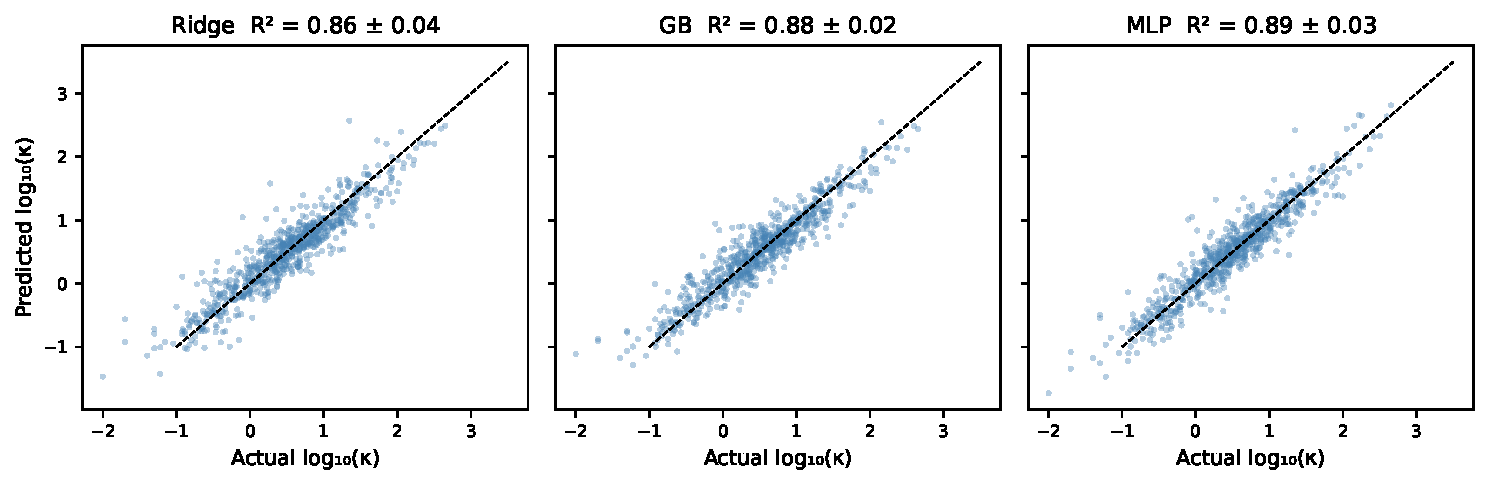
\includegraphics[width=\columnwidth]{fig1_ceiling.pdf}
\caption{Predicted vs.\ actual $\log_{10}(\kappa)$ for Ridge, gradient boosting, and neural network models with 14 harmonic features on 751 materials.}
\label{fig:ceiling}
\end{figure}

\begin{figure}
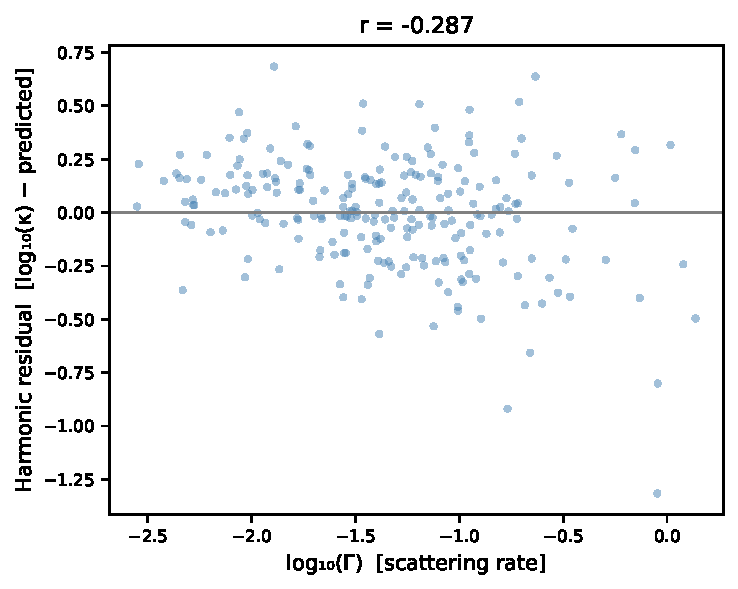
\includegraphics[width=\columnwidth]{fig2_residual.pdf}
\caption{Cross-validated (out-of-fold) harmonic residual vs.\ anharmonic scattering rate $\Gamma$ on the 231-material RTA subset.}
\label{fig:residual}
\end{figure}

\begin{figure}
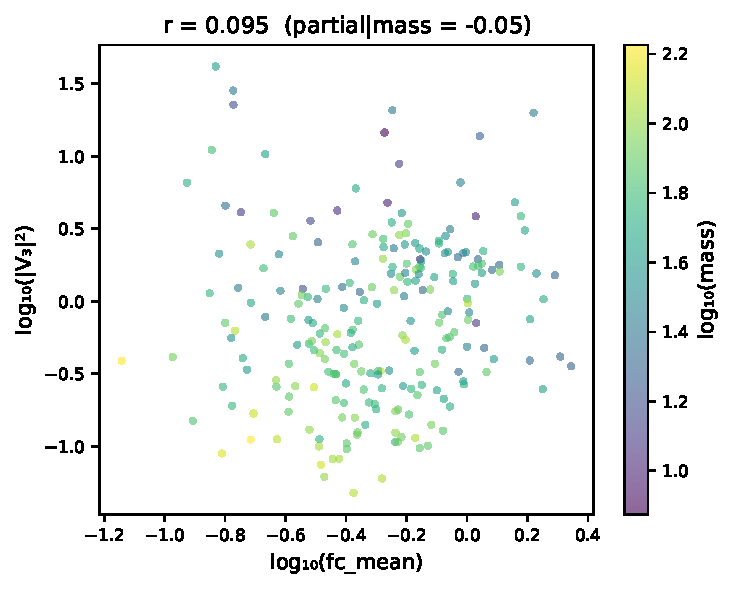
\includegraphics[width=\columnwidth]{fig3_stiffness.pdf}
\caption{Bond stiffness ($f_\mathrm{c,mean}$) vs.\ cubic coupling strength ($|V_3|^2$), colored by atomic mass. The weak raw correlation ($r = +0.09$) vanishes after mass control (partial $r = -0.05$), indicating that the apparent correlation is mass-mediated rather than intrinsic.}
\label{fig:stiffness}
\end{figure}

\begin{figure}
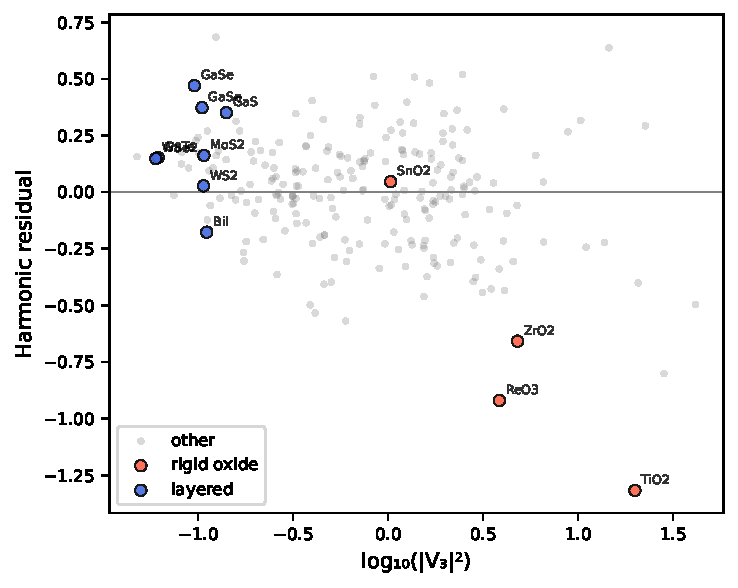
\includegraphics[width=\columnwidth]{fig4_outliers.pdf}
\caption{Harmonic residual vs.\ $|V_3|^2$ with rigid oxides (red) and layered compounds (blue) highlighted.}
\label{fig:outliers}
\end{figure}

\begin{figure}
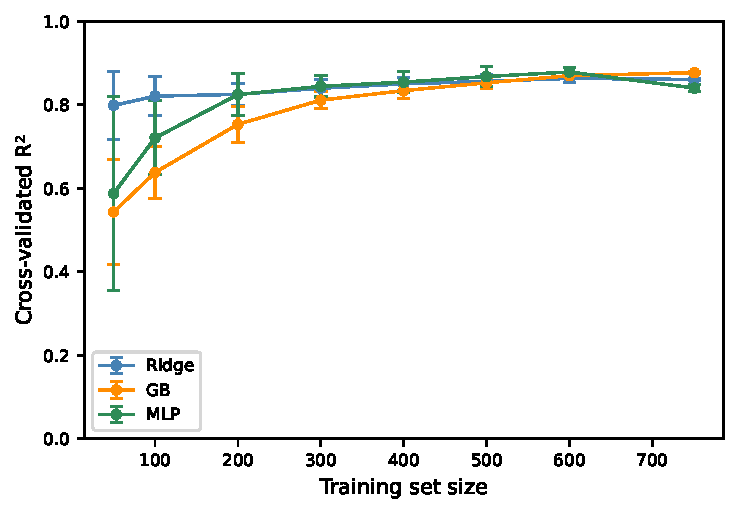
\includegraphics[width=\columnwidth]{fig5_learning.pdf}
\caption{Cross-validated $R^2$ vs.\ training set size for three model families, showing saturation by $N \approx 400$.}
\label{fig:learning}
\end{figure}

\end{document}
